\chapter{Einleitung}
\label{ch:einleitung}

DNA Sequenzierung ist aus der biologischen und medizinischen Forschung nicht mehr wegzudenken.
Die Entwicklung immer günstigerer und leistungsstärkerer Sequenzierungsverfahren hat in den letzten Jahrzenten für einen rapiden Anstieg der zu verarbeitenden Datenmengen gesorgt.
Hinzu kommt, dass die verwendeten Verfahren nicht fehlerfrei sind, was die Verarbeitung der Daten weiter erschwert.

In dieser Arbeit wird ein Paper behandelt, in dem der Fehlerkorrekturalgorithmus FMOE vorgestellt wird.
Zu erst wird aber der Hintergrund in den Bereichen Biologie und Bioinformatik erläutert.

\section{DNA-Sequenzierung}
\label{s:dna-seq} 

Das Ziel der de-novo DNA-Sequenzierung ist die Bestimmung der Nukleotidfolge in DNA ohne ein bereits bekanntes Referenzgenom.
Wo bei alten Verfahren noch alle Basen nacheinander bestimmt wurden, werden seit dem sogenannten Shotgun Sequencing viele Teilstücke der DNA parallel analysiert.
Das macht es möglich, lange DNA Stränge mit Verfahren zu sequenzieren, die nur kurze Fragmente verarbeiten können. %TODO Beispiel Illumina: 150-300bp per read
Gleichzeitig ermöglicht es die parallele Sequenzierung von mehreren Fragmenten, was den Vorgang extrem beschleunigt.

%Bild: DNA-Strang Kopien -> Fragmente -> Reads -> Assembly -> Sequenz *?Das von Wikipedia?*
% TODO: Quelle
\begin{figure}[h]
	\begin{center}
		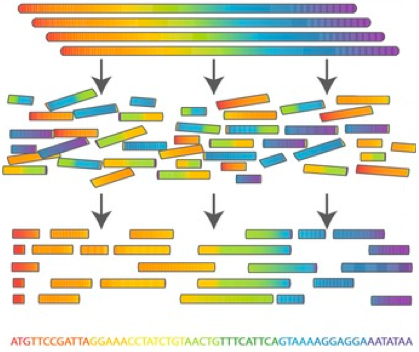
\includegraphics[width=.5\columnwidth]{./img/shotgun_sequencing.png}
	\end{center}
	\caption{Shotgun Sequenzierung: Kopien des DNA-Strangs (oben) werden an zufälligen Positionen fragmentiert und sequenziert(darunter), in die korrekte Reihenfolge gebracht (3. von oben) und zur Gesamtsequenz zusammengesetzt (unten)}
	\label{fig:shotgun-sequencing}
\end{figure}

Die Reihenfolge der DNA-Fragmente aufrecht zu erhalten, ist möglich, aber relativ langsam.
Die sogenannten next-gen Sequenzierungsverfahren, welche den aktuell höchsten Durchsatz erzielen, verzichten daher darauf.
Um trotzdem auf die ursprüngliche Reihenfolge und damit auf die gesamte DNA-Sequenz zurückschließen zu können, wird das Verfahren für mehrere Kopien desselben DNA-Strangs durchgeführt.

Wie in Abbildung \ref{fig:shotgun-sequencing} zu sehen, trennt man also mehrere Kopien des Strangs an zufälligen Positionen in ungefähr gleich lange Fragmente.
Alle Fragmente können dann unabhängig von einander - und damit parallel - sequenziert werden.
Das Ergebnis der Sequenzierung eines Fragments wird Read genannt.
Aufgrund der zufälligen Trennungspositionen überlappen sich viele dieser Reads.
Vorausgesetzt die Abdeckung\footnote{Abdeckung (Englisch Coverage) beschreibt die Anzahl einzigartiger Reads, die dieselbe Base enthalten.}
reicht an allen Stellen der Sequenz aus, kann man mit den Überlappungen die Reads in die ursprüngliche Reihenfolge bringen und so die gesuchte DNA-Sequenz bestimmen.
%Fußnote Abdeckung/Coverage
Dieser Prozess heißt Assembly.

Wie bereits erwähnt, sind die aktuellen Verfahren zur Bestimmung der Reads nicht fehlerfrei.
Es kann zum Überspringen (Deletion) oder Vertauschen (Substitution) richtiger Basen oder zur Einfügung (Insertion) falscher Basen kommen.
Kollektiv werden diese Fehler Indels genannt.

Die Assembly üblicherweise durch Überlappungsgraphen oder de Bruijn Graphen bewältigt.
Überlappungsgraphen können Fehler bis zu einem gewissen Maß kompensieren, bringen allerdings hohe Speicher- und Rechenanforderungen mit sich.
De Bruijn Graphen sind deutlich resourcensparender, tolerieren aber keine Fehler.
Aus diesem Grund wird bei großen Datenmengen oft auf de Bruijn Graphen mit vorheriger Fehlerkorrektur zurückgegriffen.

Fehler in den Reads sorgen für verschiedene Probleme bei der Assembly mithilfe eines de Bruijn Graphen:
\begin{description}
	\item[Fragmentierte Assembly]\hfill \\
		Fehlerhafte Reads verhindern das Erkennen von Überlappungen und sorgen für Graphen, die keine valide Assembly zulassen. Ein Beispiel für eine fragmentierte Assembly ist in Abbildung \ref{fig:debruijn-fragmented} zu sehen.
	\item[Misassembly]\hfill \\
		Fehlerhafte Reads überlappen sich in manchen Fällen mit korrekten Reads und sorgen für eine valide Assembly, die aber eine falsche Sequenz ergibt. \\
		Dieser Fall ist im Nachhinein schwer zu erkennen.
\end{description}
Zusätzlich erhöht sich die Komplexität des Graphen bei fehlerhaften Reads unter Umständen enorm.

%Bild: Assemblygraph mit und ohne Indels
% TODO: Quelle
\begin{figure}[h]
	\begin{center}
		\subfigure[Intakter de Bruijn Graph] {
			\makebox[.45 \columnwidth]{
				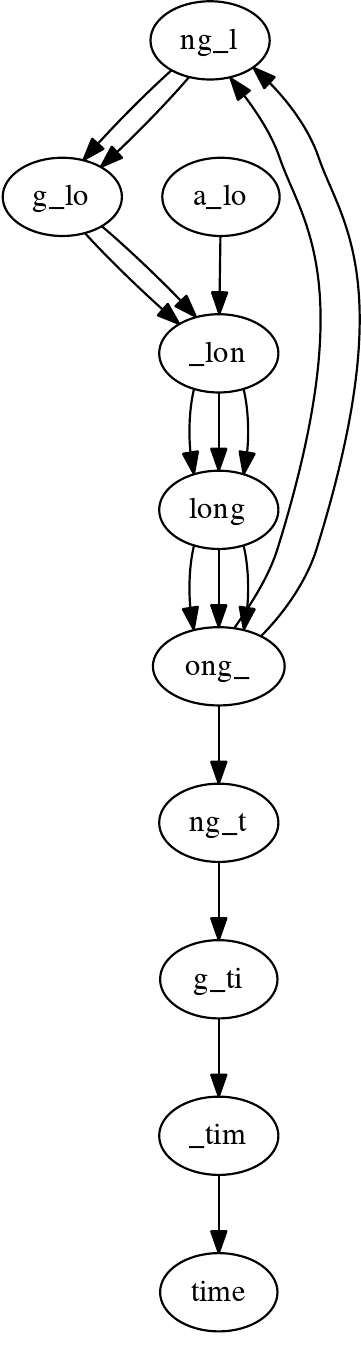
\includegraphics[scale=.75]{./img/debruijn_correct.png}
				\label{fig:debruijn-correct}
			}
		}
		\subfigure[Fragmentierter de Bruijn Graph] {
			\makebox[.45 \columnwidth]{
				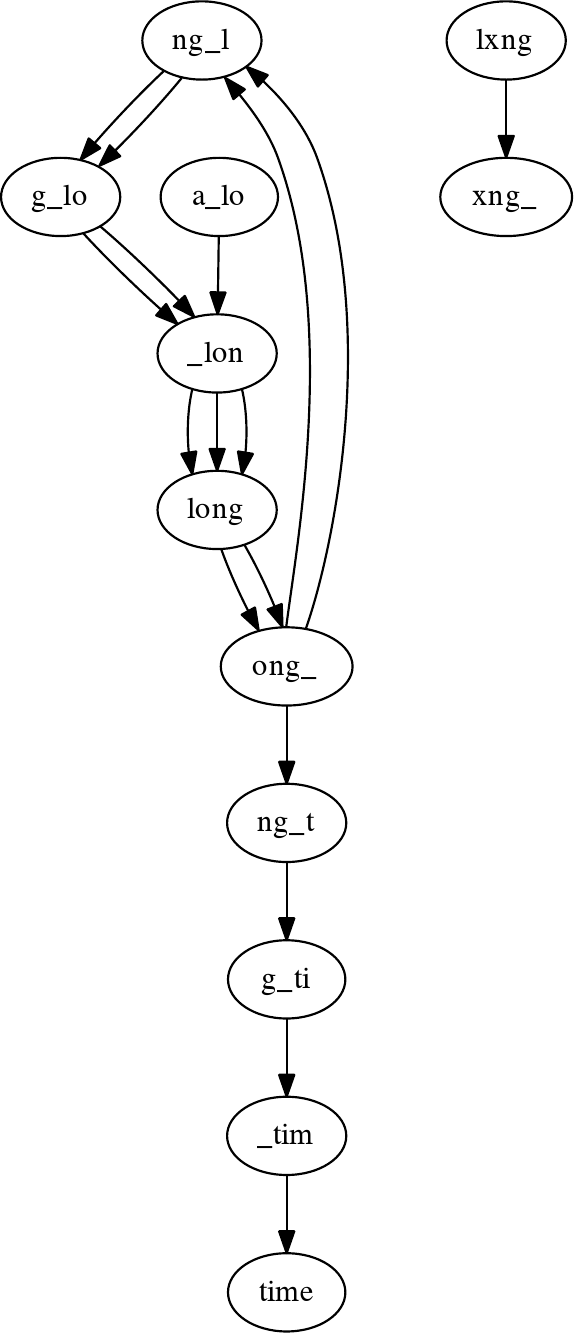
\includegraphics[scale=.75]{./img/debruijn_fragmented.png}
				\label{fig:debruijn-fragmented}
			}
		}
	\end{center}
	\caption{De Bruijn Graph des Texts \glqq a long long time\grqq . Oben der Graph aus fehlerfreien Fragmenten, unten der fragmentierte Graph, hervorgerufen durch Substitutionsfehler.}
	\label{fig:debruijn-graph}
\end{figure}


\section{Fehlerkorrektur}
\label{s:error-correction} 

Aufgabe der Fehlerkorrektur ist es, diese Komplikationen zu verhindern. \\
Da bei der de-novo Sequenzierung kein Referenzgenom zur Verfügung steht, kann die Fehlerkorrektur nur auf Grundlage der Reads geschehen.
Die üblichen Verfahren stützen sich dabei auf statistische Modelle, um fehlerhafte Reads zu finden und zu verwerfen oder zu korrigieren.

Das hier behandelte Paper teilt Fehlerkorrekturalgorithmen in drei Kategorien:
\begin{description}
	\item[k-mer Frequenzsprektrum Methoden] erzeugen eine Erhebung aller k-mere\footnote{k-mer wird eine k Zeichen lange Teilkette einer Zeichenkette genannt. Beispiel: Die 3-mere von \glqq ABCDE\grqq sind \glqq ABC\grqq \glqq BCD\grqq und \glqq CDE\grqq.}
	und ihrer Häufigkeiten aus den Reads und ersetzen seltene k-mere durch Häufige. \\
		Diese Verfahren sind empfindlich gegenüber Wiederholungen in der DNA-Sequenz.
	\item[Suffix-Tree / -Array Methoden] erzeugen einen Index der Suffixe der Reads in Form eines Arrays oder Baums und verhalten sich ansonsten ähnlich zu den k-mer-basierten Methoden. \\
		Die variable Länge der Suffixe macht diese Verfahren etwas resistenter gegen Wiederholungen.
	\item[Überlappungsbasierte Methoden] suchen für jeden zu korrigierenden Read alle überlappenden Reads und korrigieren potenzielle Fehler mit einem MSA\footnote{MSA ist die Abkürzung für Multiple Sequence Alignment und beschreibt das alignen von mehr als drei DNA-Sequenzen. Mit alignment ist an dieser Stelle der methodische Vergleich von Sequenzen gemeint.} %TODO:more?
 der gefundenen Reads. \\
		Durch die Verwendung der ganzen Reads sind diese Verfahren nicht anfällig für Wiederholungen, allerdings ist die berechnung des MSA Berechnung sehr langsam.
\end{description}
Weitere Vor- und Nachteile der verschiedenen Vorgehensweisen werden später noch erläutert. %TODO: werden sie?
